\section{はじめに}

\subsection{研究背景}
近年,深層学習は大きな発展を見せている.
Recurrent Neural Network\cite{rnn}はConvolutional Neural Network\cite{cnn}にはない
「時間」という概念を持ち,機械翻訳の分野で大きな成果を出した.
一方で,小説などの大きな入力には対応できないという欠点もあった.
RNNに長期的記憶の概念を導入したLSTM\cite{lstm}やGRU\cite{gru}も開発されたが,
計算時間の増加が問題であった.

2017年に登場したTransformer\cite{transformer}は単純な行列計算のみで完結したネットワークで,
機械翻訳でこれまでのRNNを超える精度を出し,計算時間も大幅に削減したことで,
機械翻訳のデファクトスタンダードとなった.
2020年にはVision Transformer\cite{vit}が開発され,画像認識でCNNを超える精度を出した.
さらに翌年にはVideo Vision Transformer\cite{vivit}が開発され,動画解析でもRNNを超える精度を出した.

AIの活躍は単純なタスクに留まらない.ボードゲームでは,
囲碁のAlphaGo\cite{alphago},その後継でフレームワークとして
開発されたAlphaZero\cite{alphazero}は囲碁,チェス,将棋で成果を上げた.
芸術ではMusic Transformer\cite{mut}で作曲,DALL-E2\cite{dalle2}で
図\ref{astronaut}のような作画が可能となった.

\begin{figure}[b]
  \begin{center}
    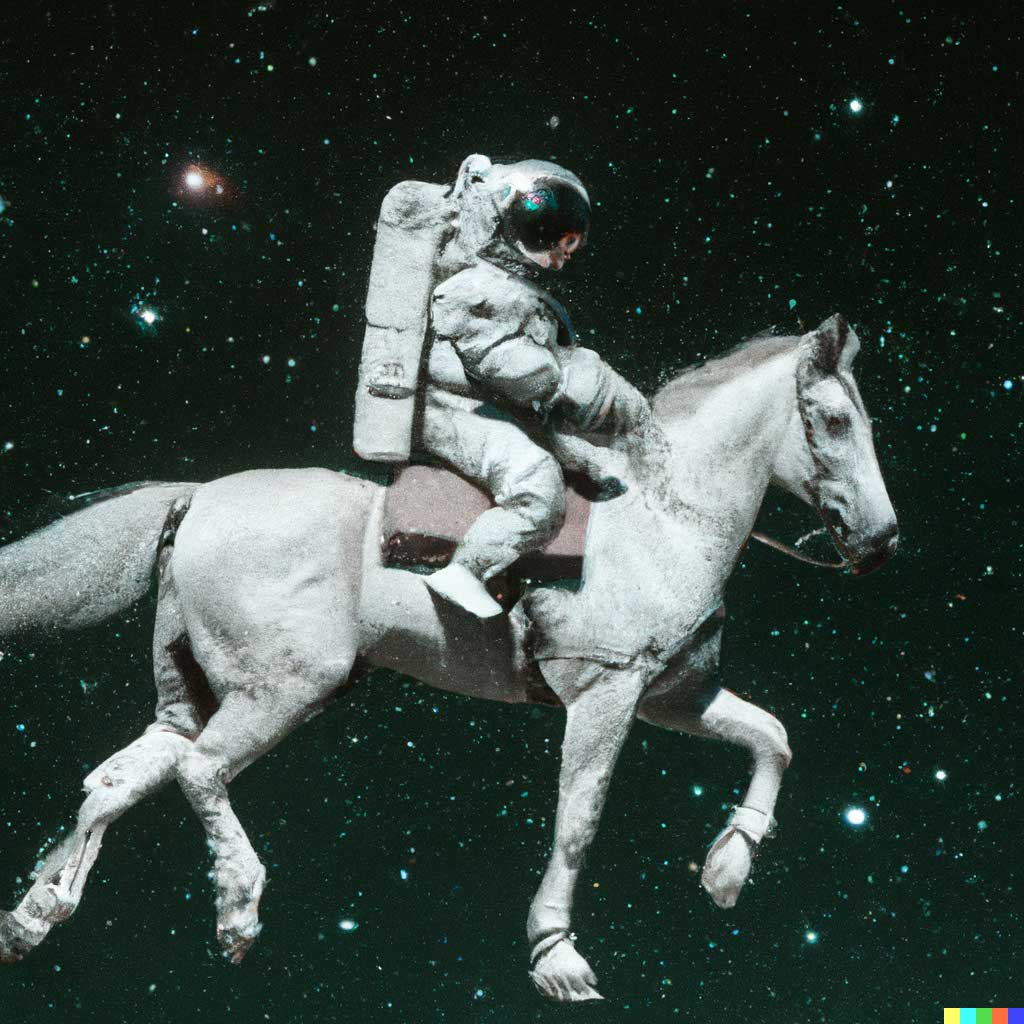
\includegraphics[width=60mm]{images/astronaut.jpg}
  \end{center}
  \caption{単語から生成されたDALL-E2の作画}
  \label{astronaut}
\end{figure}
\clearpage

「優美さ」とは,人間の動作を表現する形容詞である.
Buytendijkは,優美な動作とは
\begin{enumerate}
  \item ゆっくりとした,丸みのある動き
  \item 持続性と流動性を持つ動き
  \item 緊張と解繁がリズミカルに交替して現れる動き
\end{enumerate}
であると主張した.
また,Hogarthは,図\ref{hogarth_curve}のような「美の線」を多く含むものであると主張した.

\begin{figure}[t]
  \begin{center}
    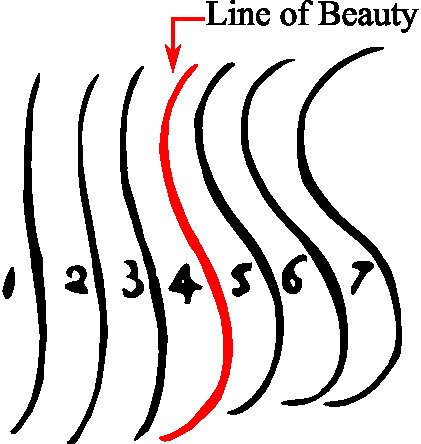
\includegraphics[width=60mm]{images/hogarth_curve.pdf}
  \end{center}
  \caption{Hogarth Curve}
  \label{hogarth_curve}
\end{figure}

単純作業,ボードゲーム,果ては芸術まで人間を凌駕するまでに成長したAI,人間の判断は
必ずしも正しいとは言えなくなってきている.「優美さ」の根底にある判断根拠とは一体どんなものなのか,
手先や足の動きにのみ囚われた解析は正しいと言えるのか,このような疑問を持った.
AIを用いて優美さを特定しようとした場合,一体どのような結果をもたらすのか,従来の結果と
どのような相違点または共通点が存在するのかを特定するために今回の研究を行った.
\clearpage

\subsection{研究目的}
我々の研究室ではHogarthの規範に則り,動作解析や動作生成を行ってきた.
稲津\cite{inadu}は手先の軌道をB-spline近似\cite{bspline}したのちに
\begin{enumerate}
  \item 軌道長がより長い
  \item Hogarth Curveとの形状類似度
  \item 両弧の弧長がほぼ等しい
  \item 両弧の全曲率が0.873〜1.44
\end{enumerate}
を検証する評価モデルを提案した.

照岡\cite{teruoka}は強化学習を用いて曲線の生成を試みた.図\ref{robot_arm}のような
シミュレータ上で駆動する仮想ロボットアームを,強化学習から生成される動作で動かした.
目標点との位置差分と各関節の加速度を用いて,照岡の提案する様々な報酬関数で学習を進めた.
それらの動作を同じくB-spline近似し,稲津の評価モデルで優美さを検証した.

\begin{figure}[b]
  \begin{center}
    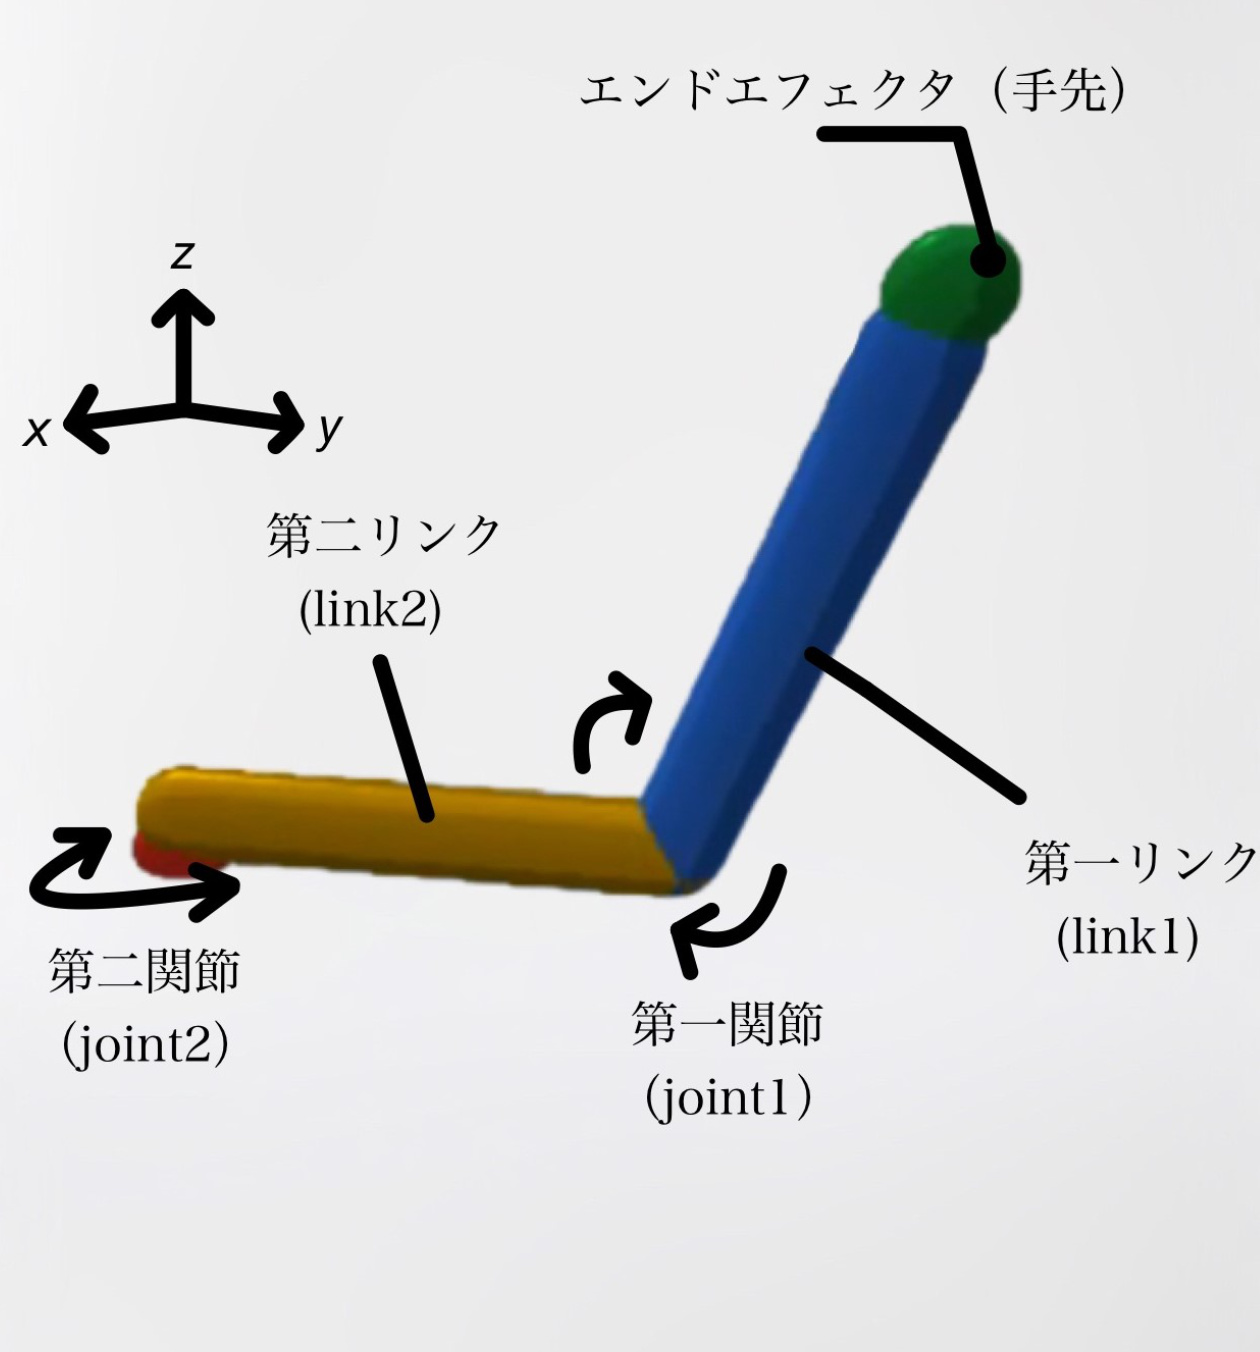
\includegraphics[width=70mm]{images/robot_arm.png}
  \end{center}
  \caption{実装した2自由度ロボットアーム}
  \label{robot_arm}
\end{figure}
\clearpage

これらの研究は手先軌道に限定して着目したもので,論文内でも他部位との関係検証の必要性や
特定状況下でしか機能しないことが言及されている.
実際,上田研では実データとして既存のcsvデータを使用するにとどまっていた.
さらに最終的な優美評価はアンケートによる主観評価で,これもデータ量として少ないものであった.

深層学習を用いることでデータに依存しないネットワーク構築が可能であり,
データが増えるほど精度が上がることが期待できる.
さらに,mp4を実データとすることでデータ収集も容易かつ大量に行うことが可能となった.
動画全体を対象とすることで目的とする網羅的検証も可能となり,これにより
従来の解析手法との比較から得られる相違点,共通点が明瞭となると考えた.

\subsection{研究構成}
第2章では開発した舞踊分類ネットワークの構造及び学習に使用した動画データを記載した.
このネットワークは動画を[優美なダンス,普通のダンス,その他の動作]に分類することを目的とするが,
通常のAIのように精度を100\%に近づけることを目指さない.
Buytendijkの定義やHogarthの定義は動作の始点から終点を観測した時に生じるものであるから,
動作が完結したと思われるまで優美であるかどうかは判断できない.
また,ダンスにはしばしば静止した状態を保つ表現技法が用いられる.
これも優美さとは動作から生まれるものと定義されているため,判断できない.
これらのため,ダンス全体,動画の内容全てを優美と決定づけることは不可能であると考えた.
その上で,動画をソフトに分類し,それぞれのエッセンスを取り出すことを試みた.

第3章では第2章で得たエッセンスを元に動画のどこから優美であるかを判断したのか検証した.
用いた手法として,Grad Cam\cite{gradcam}と確率分布を提案した.
Grad CamとはCNNの可視化手法であるCam\cite{cam}に勾配情報を追加して検証する手法である.
勾配を使用するため,画像でははっきりと見えていた判断根拠が,入力の大きな動画では
離散することが考えられる.
動画という時間に依存したデータであることと,出力がsoftmaxによる確率であることから,
動画全体の確率分布をグラフに起こし,どの辺りが確率が高まっているかを確認することで
判断根拠を特定しようとする試みも合わせて行った.

第4章では本研究の総括と今後の展望についてまとめた.